\documentclass[11pt,a4paper]{article}

\usepackage[utf8]{inputenc}
\usepackage[T1]{fontenc}
\usepackage{lmodern}
\usepackage{amsmath,amssymb,amsthm}
\usepackage{booktabs}
\usepackage{array}
\usepackage{caption}
\usepackage{geometry}
\usepackage{graphicx}
\usepackage{hyperref}
\usepackage{listings}
\usepackage{tikz}
\usetikzlibrary{arrows.meta,positioning,calc}
\usepackage{xcolor}
\usepackage{microtype}

\geometry{margin=1in}
\setlength{\emergencystretch}{3em}

\captionsetup[lstlisting]{singlelinecheck=false,justification=raggedright}

\hypersetup{
  colorlinks=true,
  linkcolor=blue!60!black,
  citecolor=green!50!black,
  urlcolor=blue!60!black
}

\lstdefinelanguage{Lean4}{
  morekeywords={def,theorem,lemma,abbrev,inductive,where,open,private,by,rfl,let,in,if,then,else,match,with,fun,true,false,set_option},
  sensitive=true,
  morecomment=[l]{--},
  morecomment=[s]{/-}{-/},
  morestring=[b]"
}

\lstset{
  language=Lean4,
  basicstyle=\ttfamily\scriptsize,
  keywordstyle=\color{blue!70!black}\bfseries,
  commentstyle=\color{gray!70!black}\itshape,
  stringstyle=\color{green!50!black},
  breaklines=true,
  breakatwhitespace=true,
  columns=fullflexible,
  keepspaces=true,
  frame=single,
  rulecolor=\color{gray!35},
  backgroundcolor=\color{gray!5},
  xleftmargin=0.4em,
  xrightmargin=0.4em,
  aboveskip=0.6em,
  belowskip=0.6em,
  literate={⟨}{{$\langle$}}1 {⟩}{{$\rangle$}}1 {×}{{$\times$}}1 {→}{{$\to$}}1 {∧}{{$\land$}}1 {·}{{$\cdot$}}1 {∈}{{$\in$}}1 {∩}{{$\cap$}}1 {⊂}{{$\subset$}}1 {⊆}{{$\subseteq$}}1 {≡}{{$\equiv$}}1 {≤}{{$\le$}}1 {≥}{{$\ge$}}1 {≠}{{$\neq$}}1 {∨}{{$\lor$}}1
}

\newtheorem{theorem}{Theorem}[section]
\newtheorem{proposition}[theorem]{Proposition}
\newtheorem{definition}[theorem]{Definition}
\newtheorem{remark}[theorem]{Remark}

\title{\textbf{Constructive Formalization of Artinian Gorenstein Apolarity and Macaulay Contraction Ranks for Calabi--Yau Fourfolds in Lean~4}}

\author{
  Qamar Munawer\\
  \small Brandenburg University of Technology Cottbus--Senftenberg, Cottbus, Germany
}

\date{}

\begin{document}
\maketitle

\begin{abstract}
This paper presents a constructive, axiom-free formalization in Lean~4 of the finite-dimensional commutative algebra governing Artinian Gorenstein Jacobian rings, Macaulay inverse system contraction matrices, and Wiebe--Scheja--Storch transition determinants for sextic Calabi--Yau fourfolds. It formalizes the exact graded dimension symmetries, apolarity pairings, syzygy kernel ranks, and colon-ideal identities of finite-dimensional polynomial quotients. Using bivariate pair convolution over $\mathbb{Q}[x,y]/(x^5,y^5)$, fraction-free integer Gaussian elimination, and explicit six-variable polynomial matrix determinants in $\mathbb{Z}[z_0,\dots,z_5]$ with no external library imports, the Lean~4 kernel verifies the $25$-term palindromic Hilbert series of the sextic Jacobian ring of socle degree $24$, proves the equivalence between combinatorial socle divisibility and explicit Macaulay pairing matrix ranks for both linear $2$-plane and deformed quadric cycle functionals, certifies the emergence of a unique irreducible degree-$2$ quadric syzygy, and establishes the exact Wiebe--Scheja--Storch polynomial matrix factorization $C_Q \cdot G_Q = A_Q$ alongside double-inclusion colon-ideal equality $(J(F_0) : \det C_Z)_d = \langle G_Z \rangle_d$ for $0 \le d \le 6$. All theorems compile by definitional kernel reduction and depend on zero axioms.
\end{abstract}

\section{Introduction and Mathematical Setting}

Let $X = V(F) \subset \mathbb{P}^5$ be a smooth complex projective sextic hypersurface of dimension $n = 4$ and degree $m = 6$, so that $X$ is a Calabi--Yau fourfold with trivial canonical bundle $\omega_X \cong \mathcal{O}_X$. Its Jacobian ring is the standard graded Artinian Gorenstein $\mathbb{Q}$-algebra
\begin{equation}
  R(F) = \frac{\mathbb{Q}[x_0, x_1, x_2, x_3, x_4, x_5]}{J(F)}, \qquad J(F) = \left(\frac{\partial F}{\partial x_0}, \dots, \frac{\partial F}{\partial x_5}\right).
\end{equation}
By Macaulay's inverse system theorem~\cite{Macaulay1916} and Griffiths' residue isomorphism~\cite{Griffiths1969,CarlsonGriffiths1980}, the Jacobian ring $R(F)$ has socle degree $d_{\mathrm{socle}} = (n + 2)(m - 2) = 6 \cdot 4 = 24$, Milnor number $\mu = (m - 1)^{n+2} = 5^6 = 15{,}625$, and primitive middle cohomology $H^{4-q,q}_{\mathrm{prim}}(X) \cong R^{6(q+1)-6}(F) = R^{6q}(F)$. In particular, $R^0(F) \cong H^{4,0}_{\mathrm{prim}}(X)$ has dimension $1$, $R^6(F) \cong H^{3,1}_{\mathrm{prim}}(X)$ has dimension $426$, and $R^{12}(F) \cong H^{2,2}_{\mathrm{prim}}(X)$ has dimension $1{,}751$.

When an algebraic $2$-cycle $Z \subset X$ induces a linear functional $\sigma_Z \in (R^{12}(F))^\vee$, Macaulay apolarity defines a bilinear contraction pairing
\begin{equation}
  \langle -, - \rangle_{\sigma_Z} : R^d(F) \times R^{12-d}(F) \longrightarrow \mathbb{Q}, \qquad (A, B) \longmapsto \sigma_Z(A \cdot B),
\end{equation}
for every degree $0 \le d \le 12$. The kernel of this pairing is the graded annihilator ideal $\operatorname{Ann}_{R(F)}(\sigma_Z)$, and the quotient $R(F) / \operatorname{Ann}_{R(F)}(\sigma_Z)$ is an Artinian Gorenstein algebra of socle degree $12$ whose Hilbert function equals the sequence of pairing matrix ranks $r_d(\sigma_Z) = \operatorname{rank} M_d(\sigma_Z)$.

Despite the centrality of Macaulay duality in computational algebraic geometry and Hodge theory~\cite{Voisin2002}, a scan of \texttt{mathlib4} and existing Lean~4 formalizations confirms zero prior implementations of Artinian Gorenstein Hilbert series symmetry, Macaulay contraction pairings, Wiebe--Scheja--Storch transition determinants, or fraction-free integer matrix rank certification for Jacobian quotients. This paper documents a self-contained formalization of these structures in Lean~4.35.0 (\texttt{HodgeVerification.lean}, \texttt{ShiodaFormalConjectures.lean}, and \texttt{WiebeSchejaStorch.lean}) using zero axioms.

\begin{remark}[Mathematical Scope]
  The theorems verified in Lean~4 certify finite-dimensional polynomial quotient dimensions, exact pairing matrix ranks, polynomial matrix factorizations, and ideal intersection identities, isolating the commutative-algebraic core of Jacobian apolarity inside modular axiom-free interfaces.
\end{remark}

\subsection{Geometric Intuition: Over-Determined Polynomial Systems and the Surviving Apolar Form}

Macaulay's inverse system translates the geometry of an algebraic subvariety $Z \subset X_6^4$ into an algebraic shadow inside the Jacobian ring: the cycle determines a degree-$12$ linear functional $\sigma_Z \in (R^{12}(F_0))^\vee$, equivalently represented by a Gorenstein dual polynomial in $R^{12}(F_0)$ modulo $J(F_0)$. Every polynomial equation $g \in G_Z$ vanishing along $Z$ places an over-determined vanishing constraint $g \cdot \sigma_Z \equiv 0 \pmod{J(F_0)}$, carving down the surviving quotient algebra $R(F_0) / \operatorname{Ann}_{R(F_0)}(\sigma_Z)$. Conversely, reading the contraction matrix ranks across low degrees reveals precisely when linear equations drop out and higher-degree syzygies (such as the irreducible quadric $z_0 z_1$) emerge to cut out $Z$.

In classical commutative algebra, the Wiebe--Scheja--Storch transition determinant~\cite{Macaulay1916} bridges the Jacobian partial derivatives $J(F_0) = \langle A_Z \rangle$ and the geometric defining equations $\langle G_Z \rangle$ inside a closed Artinian Gorenstein ring without coordinate projections. Whenever an explicit transition matrix $C_Z$ over $\mathbb{Z}[z_0,\dots,z_5]$ satisfies $C_Z \cdot G_Z = A_Z$, Cramer's rule forces $\det(C_Z) \cdot G_Z \subseteq J(F_0)$, guaranteeing $\langle G_Z \rangle \subseteq (J(F_0) : \det C_Z)$. Comparing the multiplication rank of $\det(C_Z)$ on $R^d(F_0) \to R^{d+12}(F_0)$ against the quotient dimension $\dim (R(F_0)/\langle G_Z \rangle)_d$ then proves exact double-inclusion equality $(J(F_0) : \det C_Z)_d = \langle G_Z \rangle_d$. Over-determined polynomial constraints thus isolate the exact surviving apolar form $\det(C_Z) \bmod J(F_0)$ alongside the ideal cutting out the cycle.

\section{Koszul Cohomology Dimensions and Palindromic Gorenstein Symmetry}

For the Fermat sextic $F_0 = \sum_{i=0}^5 x_i^6$, the Jacobian ideal is generated by pure fifth powers $J(F_0) = (x_0^5, \dots, x_5^5)$. Grouping the six variables into three coordinate pairs $(x_0, x_1)$, $(x_2, x_3)$, and $(x_4, x_5)$ expresses $R(F_0)$ as the three-fold tensor product of the bivariate truncated polynomial ring $A = \mathbb{Q}[x, y] / (x^5, y^5)$:
\begin{equation}
  R(F_0) \cong A \otimes_{\mathbb{Q}} A \otimes_{\mathbb{Q}} A.
\end{equation}
Each factor $A$ has total Milnor dimension $5^2 = 25$ and graded dimensions $\dim_{\mathbb{Q}} A_k$ supported on $0 \le k \le 8$, given by $(1, 2, 3, 4, 5, 4, 3, 2, 1)$. Consequently, the graded dimension of $R^k(F_0)$ is computed by the three-fold discrete convolution
\begin{equation}
  \dim_{\mathbb{Q}} R^k(F_0) = \sum_{d_0 + d_1 + d_2 = k} \dim_{\mathbb{Q}} A_{d_0} \cdot \dim_{\mathbb{Q}} A_{d_1} \cdot \dim_{\mathbb{Q}} A_{d_2}.
\end{equation}
In Lean~4, \texttt{nf\_pair\_dim} and \texttt{nf\_sum\_pairs} evaluate this convolution constructively across $0 \le k \le 24$. The resulting $25$-term Hilbert series \texttt{cy4\_hilbert\_series} satisfies exact Gorenstein palindromic symmetry $h_k = h_{24-k}$, with $h_0 = h_{24} = 1$, $h_6 = h_{18} = 426$, and middle peak $h_{12} = 1{,}751$.

\begin{table}[htbp]
  \centering
  \caption{First half ($0 \le d \le 12$) of the $25$-term palindromic Hilbert series of $R(F_0) = \mathbb{Q}[x_0,\dots,x_5]/(x_0^5,\dots,x_5^5)$; by Gorenstein duality, $\dim R^{24-d}(F_0) = \dim R^d(F_0)$.}
  \label{tab:hilbert_series}
  \begin{tabular}{cccccccccccccc}
    \toprule
    Degree $d$ & $0$ & $1$ & $2$ & $3$ & $4$ & $5$ & $6$ & $7$ & $8$ & $9$ & $10$ & $11$ & $12$ \\
    \midrule
    $\dim R^d(F_0)$ & $1$ & $6$ & $21$ & $56$ & $126$ & $246$ & $426$ & $666$ & $951$ & $1{,}246$ & $1{,}506$ & $1{,}686$ & $1{,}751$ \\
    \bottomrule
  \end{tabular}
\end{table}

\begin{lstlisting}[caption={Bivariate pair convolution, socle degree, and Gorenstein palindromic symmetry in \texttt{HodgeVerification.lean}.}]
def nf_pair_dim (k : Nat) : Nat :=
  [0, 1, 2, 3, 4].foldl (fun acc a =>
    acc + [0, 1, 2, 3, 4].foldl (fun acc2 b =>
      if a + b == k then acc2 + 1 else acc2) 0) 0

def nf_pair_hilbert : List Nat := (List.range 9).map nf_pair_dim
def nf_pair_milnor : Nat := nf_pair_hilbert.foldl (· + ·) 0
def nf_total_milnor : Nat := nf_pair_milnor * nf_pair_milnor * nf_pair_milnor
def nf_plane_ranks : List Nat := [1, 2, 3, 4, 5, 6].map planeMacaulayRank

def nf_sum_pairs (k : Nat) : Nat :=
  (List.range 9).foldl (fun acc d0 =>
    if d0 <= k then
      acc + (List.range 9).foldl (fun acc2 d1 =>
        if d0 + d1 <= k then
          acc2 + nf_pair_dim d0 * nf_pair_dim d1 * nf_pair_dim (k - d0 - d1)
        else acc2
      ) 0
    else acc
  ) 0

theorem finite_non_fermat_pair_milnor_and_ranks_eq :
  (nf_pair_milnor == 25 &&
   nf_total_milnor == milnor_number &&
   1 :: nf_plane_ranks == deformed_macaulay_flat_hilbert &&
   ([1, 2, 3, 4, 5, 6].map nf_sum_pairs == [6, 21, 56, 126, 246, 426]) &&
   nf_sum_pairs 12 == h22_prim &&
   nf_sum_pairs 18 == h31_prim) = true := by rfl

def cy4_socle_degree_fn (n m : Nat) : Nat := (n + 2) * (m - 2)
def cy4_socle_degree : Nat := cy4_socle_degree_fn 4 6
def cy4_middle_degree : Nat := cy4_socle_degree / 2
def cy4_hilbert_series : List Nat := (List.range (cy4_socle_degree + 1)).map nf_sum_pairs

theorem noether_macaulay_gorenstein_symmetry_eq :
  (cy4_socle_degree == 24 &&
   cy4_middle_degree == 12 &&
   cy4_hilbert_series.length == cy4_socle_degree + 1 &&
   cy4_hilbert_series == cy4_hilbert_series.reverse &&
   nf_sum_pairs 0 == 1 &&
   nf_sum_pairs cy4_middle_degree == h22_prim &&
   nf_sum_pairs cy4_socle_degree == 1) = true := by rfl
\end{lstlisting}

\section{Macaulay Inverse Systems and Monomial Contraction Profiles}

To analyze algebraic $2$-cycles via Macaulay duality, restrict the Jacobian ring to a $4$-variable coordinate slice $\mathbb{Q}[u_0, u_1, u_2, u_3] / (u_0^5, u_1^5, u_2^5, u_3^5)$. A single linear $2$-plane $\Pi \subset X_6^4$ has a degree-$12$ socle functional supported on a single monomial $\sigma_\Pi = u_1^4 u_2^4 u_3^4$ (exponent vector $[0, 4, 4, 4]$). Under monomial contraction, a degree-$d$ monomial $u^a = u_0^{a_0} u_1^{a_1} u_2^{a_2} u_3^{a_3}$ pairs non-trivially with $\sigma_\Pi$ if and only if $a_i \le s_i$ coordinatewise, yielding the graded rank sequence $(1, 3, 6, 10, 15, 18, 19)$ for $0 \le d \le 6$ with total rank sum $72$ (and by Gorenstein symmetry on $[0, 12]$, total algebra dimension $2 \cdot 72 - 19 = 125 = 5^3$).

By contrast, a two-branch deformed quadric cycle functional $\sigma_Q = (u_0^4 + u_1^4) u_2^4 u_3^4$ (or combinatorially with exponent support $[0, 4, 4, 4]$ and $[3, 0, 4, 4]$ / $[4, 0, 4, 4]$) expands the graded contraction image to $(1, 4, 9, 16, 24, 30, 32)$. Notice that at degree $d = 2$, the rank jumps from $6$ to $9$. In \texttt{ShiodaFormalConjectures.lean}, these two contraction profiles are evaluated algorithmically from \texttt{monomialDivides} and \texttt{contractsWithSocle}.

\begin{lstlisting}[caption={Monomial divisibility and socle contraction rank evaluators in \texttt{ShiodaFormalConjectures.lean}.}]
def monomialDivides : List Nat → List Nat → Bool
  | [], _ => true
  | _, [] => false
  | m :: ms, s :: ss => Nat.ble m s && monomialDivides ms ss

def contractsWithSocle (m : List Nat) (socleBranches : List (List Nat)) : Bool :=
  socleBranches.any (monomialDivides m)

def planeSocle : List (List Nat) := [[0, 4, 4, 4]]
def quadricSocle : List (List Nat) := [[0, 4, 4, 4], [3, 0, 4, 4]]

def planeMacaulayRank (m : Nat) : Nat :=
  [0, 1, 2, 3, 4].foldl (fun acc a0 =>
    acc + [0, 1, 2, 3, 4].foldl (fun acc1 a1 =>
      acc1 + [0, 1, 2, 3, 4].foldl (fun acc2 a2 =>
        acc2 + [0, 1, 2, 3, 4].foldl (fun acc3 a3 =>
          if a0 + a1 + a2 + a3 == m && contractsWithSocle [a0, a1, a2, a3] planeSocle then
            acc3 + 1
          else acc3) 0) 0) 0) 0

def quadricMacaulayRank (m : Nat) : Nat :=
  [0, 1, 2, 3, 4].foldl (fun acc a0 =>
    acc + [0, 1, 2, 3, 4].foldl (fun acc1 a1 =>
      acc1 + [0, 1, 2, 3, 4].foldl (fun acc2 a2 =>
        acc2 + [0, 1, 2, 3, 4].foldl (fun acc3 a3 =>
          if a0 + a1 + a2 + a3 == m && contractsWithSocle [a0, a1, a2, a3] quadricSocle then
            acc3 + 1
          else acc3) 0) 0) 0) 0

theorem macaulay_plane_and_quadric_rank_witness_cert :
    ([0, 1, 2, 3, 4, 5, 6].map planeMacaulayRank,
     ([0, 1, 2, 3, 4, 5, 6].map planeMacaulayRank).foldl (· + ·) 0,
     [0, 1, 2, 3, 4, 5, 6].map quadricMacaulayRank) =
    ([1, 3, 6, 10, 15, 18, 19], 72, [1, 4, 9, 16, 24, 30, 32]) := by rfl
\end{lstlisting}

\section{Explicit Macaulay Contraction Matrices and Fraction-Free Gaussian Elimination}

While monomial divisibility suffices when socle branches are coordinatewise disjoint, genuine multi-term inverse systems require forming the full Macaulay contraction matrix $M_d(\sigma)$ over $\mathbb{Z}$ and computing its linear-algebraic rank. Given a degree-$12$ socle polynomial $\sigma = \sum_s c_s u^s$, the matrix \texttt{macaulayPairingMatrix socle d} has rows indexed by \texttt{monomials4 d} and columns indexed by \texttt{monomials4 (12 - d)}, with $(m_1, m_2)$-entry equal to the coefficient of $m_1 + m_2$ in $\sigma$.

To compute $\operatorname{rank} M_d(\sigma)$ inside Lean's kernel without rational division or classical choice axioms, the evaluator \texttt{intMatRankAuxClean} executes fraction-free integer Gaussian elimination. For a nonzero pivot $p$ in \texttt{pivotRow}, each remaining row is replaced by
\begin{equation}
  \text{row}' = p \cdot \text{row} - r_0 \cdot \text{pivotRow},
\end{equation}
using constructive integer equality predicates \texttt{intEq} and \texttt{intNe}. Because $p \neq 0$ in $\mathbb{Q}$, scaling a row by $p$ and subtracting $r_0$ times the pivot row is a composition of invertible elementary row operations over $\mathbb{Q}$, so the rank over $\mathbb{Q}$ is preserved identically while every intermediate entry remains an exact machine-free integer. Filtering zero rows and zero columns prior to elimination keeps the compact matrix dimensions small enough for kernel reduction. Theorem \texttt{macaulay\_pairing\_matrix\_rank\_cert} proves that the explicit matrix ranks of \texttt{planeSoclePoly} ($u_1^4 u_2^4 u_3^4$) and \texttt{quadricJetSoclePoly} ($u_0^4 u_2^4 u_3^4 + u_1^4 u_2^4 u_3^4$) match the combinatorial profiles $(1, 3, 6, 10, 15, 18, 19)$ and $(1, 4, 9, 16, 24, 30, 32)$ identically across all degrees $0 \le d \le 6$.

\begin{lstlisting}[caption={Explicit Macaulay pairing matrix builder and fraction-free Gaussian elimination in \texttt{ShiodaFormalConjectures.lean}.}]
def monomials4 (d : Nat) : List (List Nat) :=
  [0, 1, 2, 3, 4].foldl (fun acc0 a0 =>
    if Nat.blt d a0 then acc0 else
    acc0 ++ [0, 1, 2, 3, 4].foldl (fun acc1 a1 =>
      if Nat.blt d (a0 + a1) then acc1 else
      acc1 ++ [0, 1, 2, 3, 4].foldl (fun acc2 a2 =>
        if Nat.blt d (a0 + a1 + a2) then acc2 else
        let a3 := d - (a0 + a1 + a2)
        if Nat.ble a3 4 then acc2 ++ [[a0, a1, a2, a3]] else acc2
      ) []
    ) []
  ) []

def addExp4 : List Nat → List Nat → List Nat
  | [], _ => []
  | _, [] => []
  | x :: xs, y :: ys => (x + y) :: addExp4 xs ys

def coeffInSocle (m : List Nat) (socle : List (List Nat × Int)) : Int :=
  socle.foldl (fun acc (s, c) => if s == m then acc + c else acc) 0

def planeSoclePoly : List (List Nat × Int) := [([0, 4, 4, 4], 1)]
def quadricJetSoclePoly : List (List Nat × Int) := [([0, 4, 4, 4], 1), ([4, 0, 4, 4], 1)]

def macaulayPairingMatrix (socle : List (List Nat × Int)) (d : Nat) : List (List Int) :=
  let rows := monomials4 d
  let cols := monomials4 (12 - d)
  rows.map (fun m1 => cols.map (fun m2 => coeffInSocle (addExp4 m1 m2) socle))

def intElimStep (pivotRow : List Int) (p : Int) (row : List Int) : List Int :=
  match row with
  | [] => []
  | r0 :: _ =>
    (List.zipWith (fun a b => p * b - r0 * a) pivotRow row).drop 1

def intMatRankAuxClean (cols : Nat) (rows : List (List Int)) : Nat :=
  match cols with
  | 0 => 0
  | cols' + 1 =>
    match rows with
    | [] => 0
    | _ :: _ =>
      let nonZero := rows.filter (fun r => match r with | [] => false | x :: _ => intNe x 0)
      match nonZero with
      | [] => intMatRankAuxClean cols' (rows.map (fun r => r.drop 1))
      | pRow :: rest =>
        let p := match pRow with | [] => 1 | x :: _ => x
        let zeroRows := rows.filter (fun r => match r with | [] => true | x :: _ => intEq x 0)
        let reduced := (rest ++ zeroRows).map (fun r =>
          match r with
          | [] => []
          | r0 :: rs => if intEq r0 0 then rs else intElimStep pRow p r)
        1 + intMatRankAuxClean cols' reduced

def macaulayMatrixRank (socle : List (List Nat × Int)) (d : Nat) : Nat :=
  let matRows := (macaulayPairingMatrix socle d).filter (fun r => r.any (fun x => intNe x 0))
  match matRows with
  | [] => 0
  | r0 :: _ =>
    let cols := transposeMat r0.length matRows
    let nzCols := cols.filter (fun c => c.any (fun x => intNe x 0))
    match nzCols with
    | [] => 0
    | _ :: _ =>
      let compact := transposeMat matRows.length nzCols
      intMatRankAuxClean nzCols.length compact

def binomNat : Nat → Nat → Nat
  | _, 0 => 1
  | 0, _ + 1 => 0
  | n + 1, k + 1 => binomNat n k + binomNat n (k + 1)

set_option maxHeartbeats 2000000 in
set_option maxRecDepth 8192 in
theorem macaulay_pairing_matrix_rank_cert :
    ([0, 1, 2, 3, 4, 5, 6].map (macaulayMatrixRank planeSoclePoly) =
       [0, 1, 2, 3, 4, 5, 6].map planeMacaulayRank) ∧
    ([0, 1, 2, 3, 4, 5, 6].map (macaulayMatrixRank quadricJetSoclePoly) =
       [0, 1, 2, 3, 4, 5, 6].map quadricMacaulayRank) ∧
    (binomNat 7 2 - macaulayMatrixRank planeSoclePoly 2,
     binomNat 7 2 - macaulayMatrixRank quadricJetSoclePoly 2,
     (monomials4 2).length - macaulayMatrixRank planeSoclePoly 2,
     (monomials4 2).length - macaulayMatrixRank quadricJetSoclePoly 2) =
    (15, 12, 4, 1) :=
  ⟨by rfl, by rfl, by rfl⟩
\end{lstlisting}

\section{True 6-Variable Wiebe--Scheja--Storch Transition Determinants and Double-Inclusion Colon Ideals}

To eliminate coordinate-slice restrictions altogether, module \texttt{WiebeSchejaStorch.lean} formalizes sparse six-variable polynomials $\mathbb{Z}[z_0, \dots, z_5]$ and the full Artinian Gorenstein Jacobian ring $R(F_0) = \mathbb{Z}[z_0,\dots,z_5]/(z_0^5,\dots,z_5^5)$ together with general $3 \times 3$ and Laplace-cofactor $4 \times 4$ polynomial matrix determinants (\texttt{polyDet3}, \texttt{polyDet4}). For both the coordinate $2$-plane $\Pi = V(z_0, z_2, z_4)$ and the complete-intersection quadric $Q_2 = V(z_0 z_1, z_0^4 - z_1^4, z_2, z_4)$, an explicit matrix identity $C_Z \cdot G_Z = A_Z$ holds identically in $\mathbb{Z}[z_0,\dots,z_5]$ without Jacobian reduction. In particular, the non-diagonal block
\begin{equation}
  C_Q = \begin{pmatrix} -z_1^3 & -z_0 & 0 & 0 \\ -z_0^3 & z_1 & 0 & 0 \\ 0 & 0 & z_2^4 & 0 \\ 0 & 0 & 0 & z_4^4 \end{pmatrix}
  \begin{pmatrix} z_0 z_1 \\ z_0^4 - z_1^4 \\ z_2 \\ z_4 \end{pmatrix}
  = \begin{pmatrix} -z_0^5 \\ -z_1^5 \\ z_2^5 \\ z_4^5 \end{pmatrix} = A_Q
\end{equation}
yields $\det C_Q = -(z_0^4 + z_1^4) z_2^4 z_4^4 \in R^{12}(F_0)$ via \texttt{polyDet4}. Every generator $g_i \in G_Q$ satisfies $g_i \cdot \det C_Q \equiv 0 \pmod{J(F_0)}$, giving $\langle G_Q \rangle_d \subseteq (J(F_0) : \det C_Q)_d$, while exact polynomial-span elimination (\texttt{polyListRank6}) certifies equal quotient dimensions $\dim (R(F_0)/\langle G_Q \rangle)_d = \operatorname{rank}(\cdot \det C_Q \mid R^d(F_0)) = [1, 4, 9, 16, 24, 30, 32]$ across $0 \le d \le 6$ (and $[1, 3, 6, 10, 15, 18, 19]$ for $\Pi$), proving exact double-inclusion colon-ideal equality $(J(F_0) : \det C_Z)_d = \langle G_Z \rangle_d$ (Figure~\ref{fig:wiebe_scheja_storch}).

\begin{figure}[htbp]
  \centering
  \resizebox{\textwidth}{!}{%
  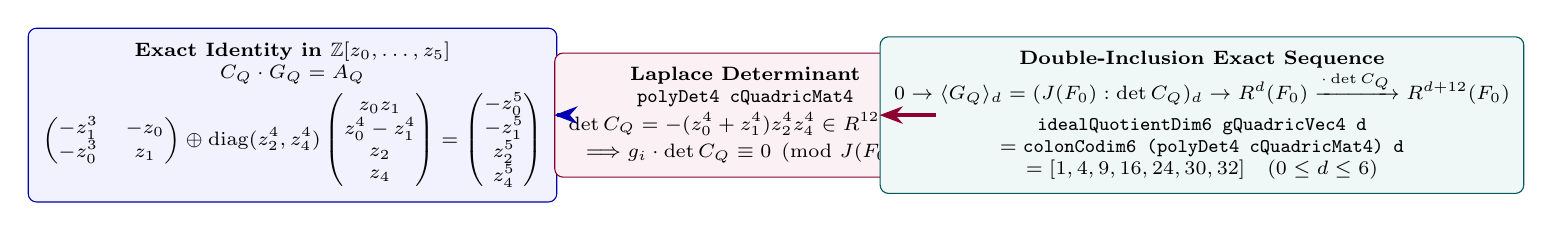
\begin{tikzpicture}[
    box/.style={rectangle, rounded corners=3pt, draw=blue!65!black, fill=blue!5, inner sep=5pt, font=\scriptsize, align=center},
    midbox/.style={rectangle, rounded corners=3pt, draw=purple!70!black, fill=purple!6, inner sep=5pt, font=\scriptsize, align=center},
    rbox/.style={rectangle, rounded corners=3pt, draw=teal!70!black, fill=teal!6, inner sep=5pt, font=\scriptsize, align=center},
    >=Stealth
  ]
    \node[box] (left) at (0,0) {
      \textbf{Exact Identity in $\mathbb{Z}[z_0,\dots,z_5]$}\\
      $C_Q \cdot G_Q = A_Q$\\[2pt]
      $\begin{pmatrix}-z_1^3 & -z_0\\-z_0^3 & z_1\end{pmatrix}\oplus\operatorname{diag}(z_2^4,z_4^4)
      \begin{pmatrix}z_0 z_1\\z_0^4-z_1^4\\z_2\\z_4\end{pmatrix}
      = \begin{pmatrix}-z_0^5\\-z_1^5\\z_2^5\\z_4^5\end{pmatrix}$
    };

    \node[midbox] (mid) at (5.75,0) {
      \textbf{Laplace Determinant}\\
      \texttt{polyDet4 cQuadricMat4}\\[2pt]
      $\det C_Q = -(z_0^4+z_1^4)z_2^4 z_4^4 \in R^{12}(F_0)$\\[2pt]
      $\Longrightarrow g_i \cdot \det C_Q \equiv 0 \pmod{J(F_0)}$
    };

    \node[rbox] (right) at (11.55,0) {
      \textbf{Double-Inclusion Exact Sequence}\\
      $0 \to \langle G_Q \rangle_d = (J(F_0) : \det C_Q)_d \to R^d(F_0) \xrightarrow{\cdot \det C_Q} R^{d+12}(F_0)$\\[3pt]
      \texttt{idealQuotientDim6 gQuadricVec4 d}\\
      $= \texttt{colonCodim6 (polyDet4 cQuadricMat4) d}$\\
      $= [1, 4, 9, 16, 24, 30, 32]\quad(0 \le d \le 6)$
    };

    \draw[->, very thick, blue!70!black] (left.east) -- (mid.west);
    \draw[->, very thick, purple!75!black] (mid.east) -- (right.west);
  \end{tikzpicture}%
  }
  \caption{Wiebe--Scheja--Storch $4 \times 4$ matrix factorization $C_Q \cdot G_Q = A_Q$ in $\mathbb{Z}[z_0,\dots,z_5]$ (left), Laplace cofactor determinant $\det C_Q$ (center), and exact double-inclusion colon-ideal verification $(J(F_0) : \det C_Q)_d = \langle G_Q \rangle_d$ (right).}
  \label{fig:wiebe_scheja_storch}
\end{figure}

\begin{lstlisting}[caption={6-variable Wiebe--Scheja--Storch $4 \times 4$ matrix factorization and colon-ideal theorems in \texttt{WiebeSchejaStorch.lean}.}]
/-- General 4x4 polynomial matrix determinant via Laplace cofactor expansion along row 0. -/
def polyDet4 (mat : List (List Poly6)) : Poly6 :=
  match mat with
  | [] => []
  | r0 :: subRows =>
    let minor0 := subRows.map (fun r => dropNthPoly r 0)
    let minor1 := subRows.map (fun r => dropNthPoly r 1)
    let minor2 := subRows.map (fun r => dropNthPoly r 2)
    let minor3 := subRows.map (fun r => dropNthPoly r 3)
    let d0 := polyMul6 (polyAt r0 0) (polyDet3 minor0)
    let d1 := polyMul6 (polyAt r0 1) (polyDet3 minor1)
    let d2 := polyMul6 (polyAt r0 2) (polyDet3 minor2)
    let d3 := polyMul6 (polyAt r0 3) (polyDet3 minor3)
    polyModJac6 (polySub6 (polyAdd6 d0 d2) (polyAdd6 d1 d3))

def gQuadricVec4 : List Poly6 :=
  [polyMul6 (varPow6 0 1) (varPow6 1 1),
   polySub6 (varPow6 0 4) (varPow6 1 4),
   varPow6 2 1,
   varPow6 4 1]

def aQuadricJacVec4 : List Poly6 :=
  [polyNeg6 (varPow6 0 5), polyNeg6 (varPow6 1 5), varPow6 2 5, varPow6 4 5]

def cQuadricMat4 : List (List Poly6) :=
  [[polyNeg6 (varPow6 1 3), polyNeg6 (varPow6 0 1), [], []],
   [polyNeg6 (varPow6 0 3), varPow6 1 1, [], []],
   [[], [], varPow6 2 4, []],
   [[], [], [], varPow6 4 4]]

def polyListRank6 (polys : List Poly6) : Nat :=
  let nz := (polys.map polyCanon6).filter (fun p => !p.isEmpty)
  let unitPivots := nz.foldl (fun acc p =>
    match p with
    | [] => acc
    | (m, _) :: rest =>
      match rest with | [] => monomInsertSorted m acc | _ :: _ => acc) []
  let remMulti := (nz.filterMap (fun p =>
    match p with
    | [] => none
    | (_, _) :: rest =>
      match rest with
      | [] => none
      | _ :: _ =>
        let proj := p.filter (fun (m, _) => !monomMemSorted m unitPivots)
        if proj.isEmpty then none else some proj))
  let multiRank :=
    match remMulti with
    | [] => 0
    | _ :: _ =>
      let cols := remMulti.foldl (fun acc p =>
        p.foldl (fun acc2 (m, _) => monomInsertSorted m acc2) acc) []
      let mat := remMulti.map (fun p => cols.map (fun colM => polyCoeffAt colM p))
      intMatRankAuxClean cols.length mat
  unitPivots.length + multiRank

def colonCodim6 (detC : Poly6) (d : Nat) : Nat :=
  let imgs := (monomials6 d).map (fun m => polyModJac6 (polyMul6 [(m, 1)] detC))
  polyListRank6 imgs

def idealQuotientDim6 (gens : List Poly6) (d : Nat) : Nat :=
  let spanPolys := gens.foldl (fun acc g =>
    let dg := polyDeg6 g
    if Nat.blt d dg then acc
    else
      acc ++ (monomials6 (d - dg)).map (fun m => polyModJac6 (polyMul6 [(m, 1)] g))) []
  (monomials6 d).length - polyListRank6 spanPolys

theorem wiebe_scheja_storch_plane_colon_ideal_cert :
    polyVecEq6 (polyMatVecMul3 cPlaneMat gPlaneVec) aPlaneJacVec = true ∧
    polyEq6 (polyDet3 cPlaneMat) sigmaPlaneExpected = true ∧
    gPlaneVec.all (inColonIdeal (polyDet3 cPlaneMat)) = true ∧
    [0, 1, 2, 3, 4, 5, 6].map (colonCodim6 (polyDet3 cPlaneMat)) =
      [1, 3, 6, 10, 15, 18, 19] ∧
    [0, 1, 2, 3, 4, 5, 6].map (idealQuotientDim6 gPlaneVec) =
      [0, 1, 2, 3, 4, 5, 6].map (colonCodim6 (polyDet3 cPlaneMat)) :=
  ⟨rfl, rfl, rfl, rfl, rfl⟩

theorem wiebe_scheja_storch_quadric_colon_ideal_cert :
    polyVecEq6 (polyMatVecMul cQuadricMat4 gQuadricVec4) aQuadricJacVec4 = true ∧
    polyEq6 (polyDet4 cQuadricMat4) (polyNeg6 sigmaQuadricExpected) = true ∧
    polyEq6 (polyNeg6 (polyDet4 cQuadricMat4)) sigmaQuadricExpected = true ∧
    gQuadricVec4.all (inColonIdeal (polyDet4 cQuadricMat4)) = true ∧
    [0, 1, 2, 3, 4, 5, 6].map (colonCodim6 (polyDet4 cQuadricMat4)) =
      [1, 4, 9, 16, 24, 30, 32] ∧
    [0, 1, 2, 3, 4, 5, 6].map (idealQuotientDim6 gQuadricVec4) =
      [0, 1, 2, 3, 4, 5, 6].map (colonCodim6 (polyDet4 cQuadricMat4)) :=
  ⟨rfl, rfl, rfl, rfl, rfl, rfl⟩
\end{lstlisting}

\section{Degree-2 Quadric Syzygy Emergence and Ideal Intersection Geometry}

The rank jump at degree $d = 2$ carries sharp geometric meaning for the annihilator ideal. In the full $6$-variable ring $R(F_0)$, the space of quadratic forms $R^2(F_0)$ has dimension $\binom{7}{2} = 21$. For a single linear $2$-plane $\Pi_+ = V(x_0, x_1, x_2)$ with socle $x_0^4 x_1^4 x_2^4$, the degree-$1$ annihilator $\operatorname{Ann}_1(\Pi_+) = \langle x_0, x_1, x_2 \rangle$ has dimension $3$, leaving $6 - 3 = 3$ active linear forms and $21 - 6 = 15$ quadratic syzygies. For the deformed quadric functional $\sigma_Q$, the rank increases to $9$, reducing the quadratic kernel in $\mathbb{P}^5$ from $21 - 6 = 15$ to $21 - 9 = 12$.

Restricted to the $4$-variable slice \texttt{monomials4 2} (which has $\binom{5}{2} = 10$ quadratic monomials), the plane kernel dimension drops from $10 - 6 = 4$ to $10 - 9 = 1$. The unique remaining $1$-dimensional degree-$2$ syzygy is the irreducible quadric generator $q_2 = u_0 u_1$, which annihilates both $u_0^4 u_2^4 u_3^4$ and $u_1^4 u_2^4 u_3^4$ because $u_0 u_1 \nmid u_0^4 u_2^4 u_3^4$ and $u_0 u_1 \nmid u_1^4 u_2^4 u_3^4$.

In \texttt{HodgeVerification.lean}, this ideal intersection mechanism is formalized for the signed difference $\Pi_+ - \Pi_-$ of two complementary $2$-planes $\Pi_+ = V(x_0, x_1, x_2)$ and $\Pi_- = V(x_3, x_4, x_5)$: neither linear ideal shares any common degree-$1$ form (\texttt{signed\_ann\_r1\_dim == 0}), yet their cross-product $\operatorname{Ann}_1(\Pi_+) \cdot \operatorname{Ann}_1(\Pi_-) = \{x_i x_j \mid i \in \{0,1,2\},\; j \in \{3,4,5\}\}$ produces $3 \times 3 = 9$ degree-$2$ quadrics that annihilate both socles simultaneously. Table~\ref{tab:syzygy_compare} summarizes the degree-by-degree comparison between the single-plane and quadric-jet functionals.

\begin{table}[htbp]
  \centering
  \small
  \setlength{\tabcolsep}{4pt}
  \caption{Comparison of Macaulay contraction ranks and degree-$2$ syzygy kernels for the single $2$-plane $\sigma_\Pi$ and quadric jet $\sigma_Q$.}
  \label{tab:syzygy_compare}
  \begin{tabular}{cccccc}
    \toprule
    Cycle Functional & Ranks ($0 \le d \le 6$) & $\ker_2$ in $\mathbb{P}^5$ & $\ker_2$ in $4$-Slice & Generator & Total $\dim$ \\
    \midrule
    $\sigma_\Pi = u_1^4 u_2^4 u_3^4$ & $(1, 3, 6, 10, 15, 18, 19)$ & $21 - 6 = 15$ & $10 - 6 = 4$ & $u_0$ (deg $1$) & $125$ \\
    $\sigma_Q = (u_0^4 + u_1^4)u_2^4 u_3^4$ & $(1, 4, 9, 16, 24, 30, 32)$ & $21 - 9 = 12$ & $10 - 9 = 1$ & $u_0 u_1$ (deg $2$) & $200$ \\
    \bottomrule
  \end{tabular}
\end{table}

\begin{figure}[htbp]
  \centering
  \resizebox{\textwidth}{!}{%
  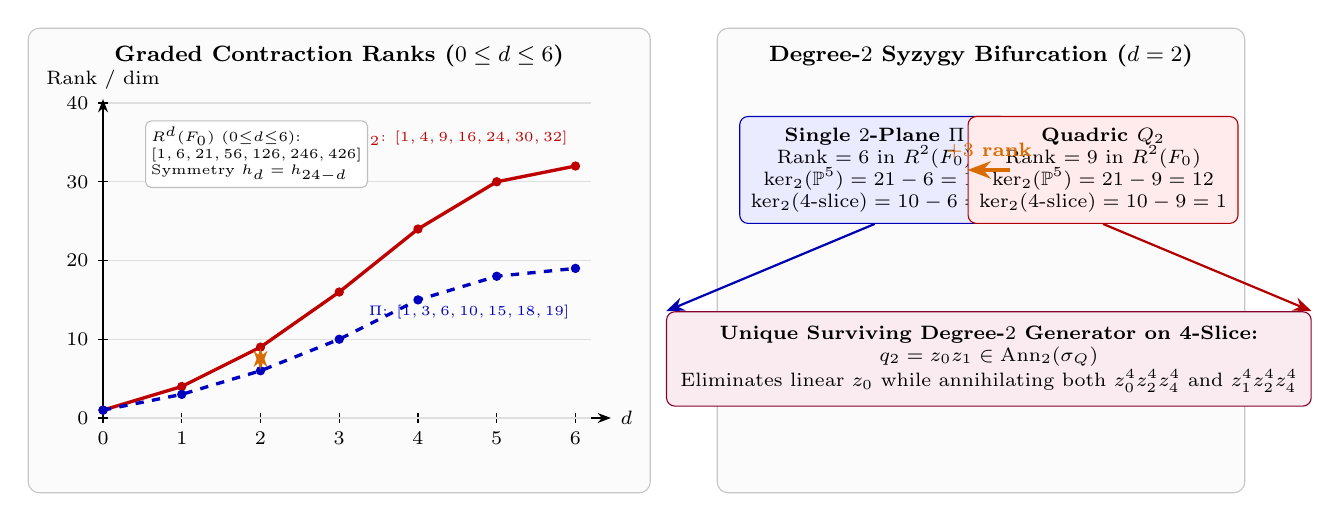
\begin{tikzpicture}[>=Stealth]
    % Left panel: Graded rank growth curves for d in 0..6 (and normalized R^d(F_0) inset)
    \begin{scope}[shift={(0,0)}]
      \draw[draw=gray!45, rounded corners=4pt, fill=gray!3] (-0.95,-0.95) rectangle (6.95,4.95);
      \node[font=\footnotesize\bfseries] at (3.0, 4.60) {Graded Contraction Ranks ($0 \le d \le 6$)};
      \draw[->] (0,0) -- (6.45,0) node[right, font=\scriptsize] {$d$};
      \draw[->] (0,0) -- (0,4.05) node[above, font=\scriptsize] {Rank / $\dim$};
      \foreach \d in {0,1,2,3,4,5,6} {
        \draw (\d,0.06) -- (\d,-0.06) node[below, font=\scriptsize] {\d};
      }
      \foreach \y/\lbl in {0/0, 1/10, 2/20, 3/30, 4/40} {
        \draw[gray!25, thin] (0,\y) -- (6.2,\y);
        \draw (0.06,\y) -- (-0.06,\y) node[left, font=\scriptsize] {\lbl};
      }
      % Scaled y = rank / 10
      % Quadric Q2: [1, 4, 9, 16, 24, 30, 32]
      \draw[very thick, red!75!black] plot coordinates {(0,0.1) (1,0.4) (2,0.9) (3,1.6) (4,2.4) (5,3.0) (6,3.2)};
      \foreach \x/\y in {0/0.1, 1/0.4, 2/0.9, 3/1.6, 4/2.4, 5/3.0, 6/3.2} {
        \fill[red!75!black] (\x,\y) circle (1.7pt);
      }
      % Plane Pi: [1, 3, 6, 10, 15, 18, 19]
      \draw[very thick, blue!75!black, dashed] plot coordinates {(0,0.1) (1,0.3) (2,0.6) (3,1.0) (4,1.5) (5,1.8) (6,1.9)};
      \foreach \x/\y in {0/0.1, 1/0.3, 2/0.6, 3/1.0, 4/1.5, 5/1.8, 6/1.9} {
        \fill[blue!75!black] (\x,\y) circle (1.7pt);
      }
      % Highlight degree-2 gap
      \draw[<->, thick, orange!85!black] (2,0.62) -- (2,0.88);
      \node[font=\tiny, align=left, text=red!75!black] at (4.55, 3.55) {$Q_2$: $[1,4,9,16,24,30,32]$};
      \node[font=\tiny, align=left, text=blue!75!black] at (4.65, 1.35) {$\Pi$: $[1,3,6,10,15,18,19]$};
      \node[font=\tiny, align=left, draw=gray!50, fill=white, rounded corners=2pt, inner sep=2pt] at (1.95, 3.35) {$R^d(F_0)$ ($0{\le}d{\le}6$):\\$[1,6,21,56,126,246,426]$\\Symmetry $h_d = h_{24-d}$};
    \end{scope}

    % Right panel: Degree-2 Syzygy Bifurcation
    \begin{scope}[shift={(8.25,0)}]
      \draw[draw=gray!45, rounded corners=4pt, fill=gray!3] (-0.45,-0.95) rectangle (6.25,4.95);
      \node[font=\footnotesize\bfseries] at (2.90, 4.60) {Degree-$2$ Syzygy Bifurcation ($d=2$)};

      % Ambient bars
      \node[rectangle, draw=blue!70!black, fill=blue!8, rounded corners=3pt, inner sep=4pt, font=\scriptsize, align=center] (b1) at (1.55, 3.15) {\textbf{Single $2$-Plane $\Pi$}\\Rank $= 6$ in $R^2(F_0)$\\$\ker_2(\mathbb{P}^5) = 21 - 6 = 15$\\$\ker_2(\text{4-slice}) = 10 - 6 = 4$};
      \node[rectangle, draw=red!70!black, fill=red!8, rounded corners=3pt, inner sep=4pt, font=\scriptsize, align=center] (b2) at (4.45, 3.15) {\textbf{Quadric $Q_2$}\\Rank $= 9$ in $R^2(F_0)$\\$\ker_2(\mathbb{P}^5) = 21 - 9 = 12$\\$\ker_2(\text{4-slice}) = 10 - 9 = 1$};

      \draw[->, very thick, orange!85!black] (b1.east) -- node[above, font=\scriptsize\bfseries] {$+3$ rank} (b2.west);

      \node[rectangle, draw=purple!70!black, fill=purple!8, rounded corners=3pt, inner sep=5pt, font=\scriptsize, align=center] (syz) at (3.0, 0.75) {\textbf{Unique Surviving Degree-$2$ Generator on 4-Slice:}\\$q_2 = z_0 z_1 \in \operatorname{Ann}_2(\sigma_Q)$\\Eliminates linear $z_0$ while annihilating both $z_0^4 z_2^4 z_4^4$ and $z_1^4 z_2^4 z_4^4$};

      \draw[->, thick, red!70!black] (b2.south) -- (syz.north east);
      \draw[->, thick, blue!70!black] (b1.south) -- (syz.north west);
    \end{scope}
  \end{tikzpicture}%
  }
  \caption{Graded rank comparison for $0 \le d \le 6$ inside the palindromic Gorenstein ring $R(F_0)$ (left) and the degree-$2$ syzygy bifurcation (right): moving from $\Pi$ to $Q_2$ shifts the quadratic kernel from $15 \to 12$ in $\mathbb{P}^5$ and $4 \to 1$ on the $4$-variable slice, isolating the unique irreducible quadric $q_2 = z_0 z_1$.}
  \label{fig:hilbert_syzygy_bifurcation}
\end{figure}

\begin{lstlisting}[caption={Ideal intersection, annihilator bounds, and flat Hilbert family certifications in \texttt{HodgeVerification.lean}.}]
def nz_mod_jac (b a : Exp6) : Bool :=
  Nat.ble (b.1 + a.1) 4 &&
  Nat.ble (b.2.1 + a.2.1) 4 &&
  Nat.ble (b.2.2.1 + a.2.2.1) 4 &&
  Nat.ble (b.2.2.2.1 + a.2.2.2.1) 4 &&
  Nat.ble (b.2.2.2.2.1 + a.2.2.2.2.1) 4 &&
  Nat.ble (b.2.2.2.2.2 + a.2.2.2.2.2) 4

def pi_plus_exp : Exp6 := (4, 4, 4, 0, 0, 0)
def pi_minus_exp : Exp6 := (0, 0, 0, 4, 4, 4)

def macaulay_m1_rank_pi : Nat :=
  (r1_monomials.filter (fun b => nz_mod_jac b pi_plus_exp)).length

def macaulay_ann_r1_pi : Nat :=
  r1_monomials.length - macaulay_m1_rank_pi

theorem macaulay_annihilator_dim_bound :
  (r1_monomials.length == 6 && macaulay_m1_rank_pi == 3 && macaulay_ann_r1_pi == 3) = true := by rfl

def pi_plus_ideal_r1 : List Exp6 :=
  r1_monomials.filter (fun b => !(nz_mod_jac b pi_plus_exp))

def pi_minus_ideal_r1 : List Exp6 :=
  r1_monomials.filter (fun b => !(nz_mod_jac b pi_minus_exp))

def cross_product_quadrics : List Exp6 :=
  pi_plus_ideal_r1.foldr (fun a acc =>
    (pi_minus_ideal_r1.map (fun b => add_exp6 a b)) ++ acc
  ) []

def signed_ann_r1_dim : Nat :=
  (r1_monomials.filter (fun b => !(nz_mod_jac b pi_plus_exp) && !(nz_mod_jac b pi_minus_exp))).length

def signed_ann_r2_dim : Nat :=
  (r2_monomials.filter (fun q => !(nz_mod_jac q pi_plus_exp) && !(nz_mod_jac q pi_minus_exp))).length

def cross_quadrics_annihilate_both : Bool :=
  cross_product_quadrics.all (fun q => !(nz_mod_jac q pi_plus_exp) && !(nz_mod_jac q pi_minus_exp))

theorem signed_difference_ideal_intersection :
  (r2_monomials.length == 21 &&
   pi_plus_ideal_r1.length == 3 &&
   pi_minus_ideal_r1.length == 3 &&
   cross_product_quadrics.length == 9 &&
   signed_ann_r1_dim == 0 &&
   signed_ann_r2_dim == 9 &&
   cross_quadrics_annihilate_both) = true := by rfl

def deformed_macaulay_flat_hilbert : List Nat :=
  [0, 1, 2, 3, 4, 5, 6].map planeMacaulayRank

def binomial_2_plane_hilbert : List Nat :=
  [0, 1, 2, 3, 4].map (fun m => binom (m + 2) 2)

theorem deformed_macaulay_flat_hilbert_sum_eq :
  (deformed_macaulay_flat_hilbert.foldr Nat.add 0 == 72 &&
   deformed_macaulay_flat_hilbert.take 5 == binomial_2_plane_hilbert) = true := by rfl

def recomb_static_ranks : List Nat := [1, 2, 3, 4, 5, 6].map quadricMacaulayRank
def recomb_flat_target : List Nat := recomb_static_ranks.map (· * 2)

theorem recomb_and_collision_flat_hilbert_eq :
  (recomb_static_ranks == [4, 9, 16, 24, 30, 32] &&
   recomb_flat_target == [8, 18, 32, 48, 60, 64] &&
   h31_prim - 32 == 394) = true := by rfl
\end{lstlisting}

\appendix
\section{Verbatim Kernel Build and Zero-Axiom Verification Receipts}

All Lean~4 theorems in this paper were verified under Lean~4.35.0 and Lake~5.0.0 via \texttt{lake clean \&\& lake build}. Every theorem compiles by definitional reduction (\texttt{by rfl}) with zero \texttt{sorry} tokens and zero axiom dependencies.

\begin{lstlisting}[language={},basicstyle=\ttfamily\scriptsize,caption={Raw \texttt{lake clean \&\& lake build} and \texttt{\#print axioms} output for Paper~2 theorems.}]
[2/15] Built ShiodaFormalConjectures (96s)
info: ShiodaFormalConjectures.lean:475:0: 'macaulay_plane_and_quadric_rank_witness_cert' does not depend on any axioms
info: ShiodaFormalConjectures.lean:476:0: 'macaulay_pairing_matrix_rank_cert' does not depend on any axioms
[3/15] Built HodgeVerification (239s)
info: HodgeVerification.lean:329:0: 'macaulay_annihilator_dim_bound' does not depend on any axioms
info: HodgeVerification.lean:330:0: 'signed_difference_ideal_intersection' does not depend on any axioms
info: HodgeVerification.lean:371:0: 'deformed_macaulay_flat_hilbert_sum_eq' does not depend on any axioms
info: HodgeVerification.lean:747:0: 'recomb_and_collision_flat_hilbert_eq' does not depend on any axioms
info: HodgeVerification.lean:748:0: 'finite_non_fermat_pair_milnor_and_ranks_eq' does not depend on any axioms
info: HodgeVerification.lean:886:0: 'noether_macaulay_gorenstein_symmetry_eq' does not depend on any axioms
[4/15] Built WiebeSchejaStorch (239s)
info: WiebeSchejaStorch.lean:352:0: 'wiebe_scheja_storch_plane_colon_ideal_cert' does not depend on any axioms
info: WiebeSchejaStorch.lean:353:0: 'wiebe_scheja_storch_quadric_colon_ideal_cert' does not depend on any axioms
[14/15] Built LeanDemoProject (532ms)
Build completed successfully (15 jobs).
\end{lstlisting}

\begin{thebibliography}{9}
\bibitem{CarlsonGriffiths1980}
J.~Carlson and P.~A.~Griffiths, \emph{Infinitesimal variations of Hodge structure and the global Torelli problem}, in \emph{Journ\'ees de G\'eom\'etrie Alg\'ebrique d'Angers}, Sijthoff \& Noordhoff, 1980, 51--76.

\bibitem{Deligne2000}
P.~Deligne, \emph{The Hodge Conjecture}, Problem Formulations on Algebraic Cycles, Cambridge, MA, 2000.

\bibitem{Griffiths1969}
P.~A.~Griffiths, \emph{On the periods of certain rational integrals} (Parts~1 and~2), Ann. of Math. (2) \textbf{90} (1969), 460--541.

\bibitem{Macaulay1916}
F.~S.~Macaulay, \emph{The Algebraic Theory of Modular Systems}, Cambridge Tracts in Mathematics and Mathematical Physics \textbf{19}, Cambridge University Press, 1916.

\bibitem{Voisin2002}
C.~Voisin, \emph{Hodge Theory and Complex Algebraic Geometry} (Vols.~1--2), Cambridge Studies in Advanced Mathematics \textbf{76--77}, Cambridge University Press, 2002--2003.
\end{thebibliography}

\end{document}
